
%%%%%%%%%%%%%%%%%%%%%%%%%%%%%%%%%%%%%%%%%
% Programming/Coding Assignment
% LaTeX Template
%
% This template has been downloaded from:
% http://www.latextemplates.com
%
% Original author:
% Ted Pavlic (http://www.tedpavlic.com)
%
% Note:
% The \lipsum[#] commands throughout this template generate dummy text
% to fill the template out. These commands should all be removed when 
% writing assignment content.
%
% This template uses a Perl script as an example snippet of code, most other
% languages are also usable. Configure them in the "CODE INCLUSION 
% CONFIGURATION" section.
%
%%%%%%%%%%%%%%%%%%%%%%%%%%%%%%%%%%%%%%%%%

%----------------------------------------------------------------------------------------
%	PACKAGES AND OTHER DOCUMENT CONFIGURATIONS
%----------------------------------------------------------------------------------------



\documentclass{article}

\usepackage{fancyhdr} % Required for custom headers
\usepackage{lastpage} % Required to determine the last page for the footer
\usepackage{extramarks} % Required for headers and footers
\usepackage[usenames,dvipsnames]{color} % Required for custom colors
\usepackage{graphicx} % Required to insert images
\usepackage{listings} % Required for insertion of code
\usepackage{courier} % Required for the courier font
\usepackage{lipsum} % Used for inserting dummy 'Lorem ipsum' text into the template
\usepackage{setspace}
\usepackage{color}
\usepackage{comment}
\usepackage{caption}
\usepackage[T1]{fontenc}
\usepackage{hyperref}
%\usepackage{natbib}
\usepackage{underscore}
\usepackage{subfigure}
\usepackage{fixltx2e}

\hypersetup{
    colorlinks=true,
    linkcolor=blue,
    filecolor=magenta,      
    urlcolor=cyan,
    breaklinks=true
}

\usepackage[]{algorithm2e}
\usepackage{pdfpages}
\usepackage{tikz}




%For python inclusion (http://widerin.org/blog/syntax-highlighting-for-python-scripts-in-latex-documents)
\definecolor{Code}{rgb}{0,0,0}
\definecolor{Decorators}{rgb}{0.5,0.5,0.5}
\definecolor{Numbers}{rgb}{0.5,0,0}
\definecolor{MatchingBrackets}{rgb}{0.25,0.5,0.5}
\definecolor{Keywords}{rgb}{0,0,1}
\definecolor{self}{rgb}{0,0,0}
\definecolor{Strings}{rgb}{0,0.63,0}
\definecolor{Comments}{rgb}{0,0.63,1}
\definecolor{Backquotes}{rgb}{0,0,0}
\definecolor{Classname}{rgb}{0,0,0}
\definecolor{FunctionName}{rgb}{0,0,0}
\definecolor{Operators}{rgb}{0,0,0}
\definecolor{Background}{rgb}{0.98,0.98,0.98}

% Margins
\topmargin=-0.45in
\evensidemargin=0in
\oddsidemargin=0in
\textwidth=6.5in
\textheight=9.0in
\headsep=0.25in

\linespread{1.1} % Line spacing

% Set up the header and footer
\pagestyle{fancy}
\lhead{\hmwkAuthorName} % Top left header
\chead{\hmwkClass\ (\hmwkClassInstructor\ \hmwkClassTime): \hmwkTitle} % Top center head
\chead{\hmwkClass\ (\hmwkClassInstructor): \hmwkTitle} % Top center head
\rhead{\firstxmark} % Top right header
\lfoot{\lastxmark} % Bottom left footer
\cfoot{} % Bottom center footer
\rfoot{Page\ \thepage\ of\ \protect\pageref{LastPage}} % Bottom right footer
\renewcommand\headrulewidth{0.4pt} % Size of the header rule
\renewcommand\footrulewidth{0.4pt} % Size of the footer rule

\setlength\parindent{0pt} % Removes all indentation from paragraphs

%----------------------------------------------------------------------------------------
%	CODE INCLUSION CONFIGURATION
%----------------------------------------------------------------------------------------

\definecolor{MyDarkGreen}{rgb}{0.0,0.4,0.0} % This is the color used for comments
\lstloadlanguages{Perl} % Load Perl syntax for listings, for a list of other languages supported see: ftp://ftp.tex.ac.uk/tex-archive/macros/latex/contrib/listings/listings.pdf
\lstset{language=Perl, % Use Perl in this example
        frame=single, % Single frame around code
        basicstyle=\small\ttfamily, % Use small true type font
        keywordstyle=[1]\color{Blue}\bf, % Perl functions bold and blue
        keywordstyle=[2]\color{Purple}, % Perl function arguments purple
        keywordstyle=[3]\color{Blue}\underbar, % Custom functions underlined and blue
        identifierstyle=, % Nothing special about identifiers                                         
        commentstyle=\usefont{T1}{pcr}{m}{sl}\color{MyDarkGreen}\small, % Comments small dark green courier font
        stringstyle=\color{Purple}, % Strings are purple
        showstringspaces=false, % Don't put marks in string spaces
        tabsize=5, % 5 spaces per tab
        %
        % Put standard Perl functions not included in the default language here
        morekeywords={rand},
        %
        % Put Perl function parameters here
        morekeywords=[2]{on, off, interp},
        %
        % Put user defined functions here
        morekeywords=[3]{test},
       	%
        morecomment=[l][\color{Blue}]{...}, % Line continuation (...) like blue comment
        numbers=left, % Line numbers on left
        firstnumber=1, % Line numbers start with line 1
        numberstyle=\tiny\color{Blue}, % Line numbers are blue and small
        stepnumber=5 % Line numbers go in steps of 5
}

% Creates a new command to include a perl script, the first parameter is the filename of the script (without .pl), the second parameter is the caption
\newcommand{\perlscript}[2]{
\begin{itemize}
\item[]\lstinputlisting[caption=#2,label=#1]{#1.pl}
\end{itemize}
}


%----------------------------------------------------------------------------------------
%	DOCUMENT STRUCTURE COMMANDS
%	Skip this unless you know what you're doing
%----------------------------------------------------------------------------------------

% Header and footer for when a page split occurs within a problem environment
\newcommand{\enterProblemHeader}[1]{
\nobreak\extramarks{#1}{#1 continued on next page\ldots}\nobreak
\nobreak\extramarks{#1 (continued)}{#1 continued on next page\ldots}\nobreak
}

% Header and footer for when a page split occurs between problem environments
\newcommand{\exitProblemHeader}[1]{
\nobreak\extramarks{#1 (continued)}{#1 continued on next page\ldots}\nobreak
\nobreak\extramarks{#1}{}\nobreak
}

\setcounter{secnumdepth}{0} % Removes default section numbers
\newcounter{homeworkProblemCounter} % Creates a counter to keep track of the number of problems

\newcommand{\homeworkProblemName}{}
\newenvironment{homeworkProblem}[1][Problem \arabic{homeworkProblemCounter}]{ % Makes a new environment called homeworkProblem which takes 1 argument (custom name) but the default is "Problem #"
\stepcounter{homeworkProblemCounter} % Increase counter for number of problems
\renewcommand{\homeworkProblemName}{#1} % Assign \homeworkProblemName the name of the problem
\section{\homeworkProblemName} % Make a section in the document with the custom problem count
\enterProblemHeader{\homeworkProblemName} % Header and footer within the environment
}{
\exitProblemHeader{\homeworkProblemName} % Header and footer after the environment
}

\newcommand{\problemAnswer}[1]{ % Defines the problem answer command with the content as the only argument
\noindent\framebox[\columnwidth][c]{\begin{minipage}{0.98\columnwidth}#1\end{minipage}} % Makes the box around the problem answer and puts the content inside
}

\newcommand{\homeworkSectionName}{}
\newenvironment{homeworkSection}[1]{ % New environment for sections within homework problems, takes 1 argument - the name of the section
\renewcommand{\homeworkSectionName}{#1} % Assign \homeworkSectionName to the name of the section from the environment argument
\subsection{\homeworkSectionName} % Make a subsection with the custom name of the subsection
\enterProblemHeader{\homeworkProblemName\ [\homeworkSectionName]} % Header and footer within the environment
}{
\enterProblemHeader{\homeworkProblemName} % Header and footer after the environment
}

%----------------------------------------------------------------------------------------
%	NAME AND CLASS SECTION
%----------------------------------------------------------------------------------------

\newcommand{\hmwkTitle}{Assignment\ \#7 } % Assignment title
%\newcommand{\hmwkDueDate}{Monday,\ January\ 1,\ 2012} % Due date
\newcommand{\hmwkClass}{Web Science} % Course/class
%\newcommand{\hmwkClassTime}{10:30am} % Class/lecture time
\newcommand{\hmwkClassInstructor}{Alexander Nwala} % Teacher/lecturer
\newcommand{\hmwkAuthorName}{Apurva Modi} % Your name

%----------------------------------------------------------------------------------------
%	TITLE PAGE
%----------------------------------------------------------------------------------------

\title{
\vspace{2in}
\textmd{\textbf{\hmwkClass:\ \hmwkTitle}}\\
%\normalsize\vspace{0.1in}\small{Due\ on\ \hmwkDueDate}\\
%\vspace{0.1in}\large{\textit{\hmwkClassInstructor\ \hmwkClassTime}}
\vspace{0.1in}\large{\textit{\hmwkClassInstructor}}
\vspace{3in}
}

\author{\textbf{\hmwkAuthorName}}
\date{Wednesday, May 1, 2019} % Insert date here if you want it to appear below your name

%----------------------------------------------------------------------------------------

\begin{document}

\maketitle
\newpage



%----------------------------------------------------------------------------------------
%	TABLE OF CONTENTS
%----------------------------------------------------------------------------------------

%\setcounter{tocdepth}{1} % Uncomment this line if you don't want subsections listed in the ToC

\newpage
\tableofcontents
\newpage

%----------------------------------------------------------------------------------------
%	PROBLEM 1
%----------------------------------------------------------------------------------------

% To have just one problem per page, simply put a \clearpage after each problem

\begin{homeworkProblem}

Create a blog-term matrix.  Start by grabbing 100 blogs; include:
\begin{verbatim}
http://f-measure.blogspot.com/
http://ws-dl.blogspot.com/
\end{verbatim}

and grab 98 more as per the method shown in class.  Note that this method randomly chooses blogs and each student will separately do
this process, so it is unlikely that these 98 blogs will be shared among students.  In other words, no sharing of blog data. Upload
to github your code for grabbing the blogs and provide a list of blog URIs, both in the report and in github.\\

Use the blog title as the identifier for each blog (and row of the matrix).  Use the terms from every item/title (RSS) or entry/title
(Atom) for the columns of the matrix.  The values are the frequency of occurrence.  Essentially you are replicating the format of the
"blogdata.txt" file included with the PCI book code.  Limit the number of terms to the most "popular" (i.e., frequent) 1000 terms,
this is *after* the criteria on p. 32 (slide 8) has been satisfied. Remember that blogs are paginated.\\
 
%\problemAnswer{

 \textbf{SOLUTION :}\\
 
  \begin{enumerate}
 	 \item\textbf{} I have used the following link to extract the blogs 
	 \begin{verbatim}
	 http://www.blogger.com/profile-find.g?t=m&q= + query (which is food in my case)
	 \end{verbatim}
  	\item\textbf{}  Created a python script \textbf{1/Assignment7_1.py} to crawl and get 104 blog URLs related to food.
	 \item\textbf{}  Added the given two blogs in to the file blogList.txt.   
	  \item\textbf{} Created the python script \textbf{1/blogData.py} to iterate through the URLs from the Outputs/blogList.txtl\\ 
	  \item\textbf{} Finally, the same script \textbf{1/blogData.py} is used to create the  \textbf{blogdata.txt} showing the blog matrix for extracted blogs.
 \end{enumerate}
 
 \begin{lstlisting}[language=Python, caption=Assignment7_1.py]
 
 import os
import requests
from bs4 import BeautifulSoup
from bs4.element import Comment

def fetch_blogs(query, limit):
    list_blogger_profiles = []
    list_blogger_urls = []
    output_directory = "Outputs/"
    blogger_url = "http://www.blogger.com/profile-find.g?t=m&q=" + query
    if not os.path.isdir(output_directory):
        os.mkdir(output_directory)
    while len(list_blogger_urls) < limit:
        response = requests.get(blogger_url)
        print(blogger_url)
        if response.status_code == 200:
            soup = BeautifulSoup(response.text, 'html.parser')
            profiles_tag_selector = soup.find_all('dl')
            for tags in profiles_tag_selector:
                profile_url_selector = tags.find('a', href=True)
                blogger_profile_url = "http://www.blogger.com/" + profile_url_selector['href'][1:]
                list_blogger_profiles.append(blogger_profile_url)
            list_blogger_urls.extend(fetch_blog_urls(list_blogger_profiles, limit))
            print(list_blogger_urls)
            list_blogger_profiles = []
            blogger_url_selector = soup.find('a', {'id': 'next-btn'},
                                             href=True)
            if blogger_url_selector:
                blogger_url = blogger_url_selector['href']
            else:
                break
            print(len(list_blogger_urls))
    print(len(list_blogger_urls))
    if os.path.isfile(output_directory + "test1.txt"):
        file_blog_urls = open(output_directory + "blogList.txt", "a+")
    else:
        file_blog_urls = open(output_directory + "blogList.txt", "w")
    for urls in list_blogger_urls:
        file_blog_urls.write(urls + "\n")
    file_blog_urls.close()

def fetch_blog_urls(list_blogger_profiles, limit):
    count = 0
    list_blogger_urls = []
    for profile in list_blogger_profiles:
        if count < limit:
            response = requests.get(profile)
            if response.status_code == 200:
                soup = BeautifulSoup(response.text, 'html.parser')
                profile_blog_link_selector = soup.find_all('span', dir=True)
                for profile_blog_links in profile_blog_link_selector:
                    if profile_blog_links['dir'] == 'ltr':
                        blog_links_selector = profile_blog_links.find_all('a', href=True)
                        for blog_links in blog_links_selector:
                            print(blog_links['href'])
                            try:
                                response = requests.head(blog_links['href'], timeout=60)
                                print(response.headers)
                                if response.encoding and (response.encoding == 'ISO-8859-1' or response.encoding == 'UTF-8'):
                                    list_blogger_urls.append(blog_links['href'])
                                    print()
                                    count += 1
                            except Exception as e:
                                print(e)
    print(list_blogger_urls)
    return list_blogger_urls

fetch_blogs("Food", 100)
file_open = open("Outputs/blogList.txt", "a+")
file_open.write("http://f-measure.blogspot.com/" + "\n")
file_open.write("http://ws-dl.blogspot.com/" + "\n")
file_open.close()

\end{lstlisting}

\newpage

\begin{lstlisting}[language=Python, caption=blogData.py]

import feedparser
import re
import urllib.parse
import requests
from bs4 import BeautifulSoup as bs4

def getwordcounts(url):
    '''
    Returns title and dictionary of word counts for an RSS feed
    '''
    # Parse the feed
    d = feedparser.parse(url)
    wc = {}
    # Loop over all the entries
    for e in d.entries:
        if 'summary' in e:
            summary = e.summary
        else:
            summary = e.description
        # Extract a list of words
        words = getwords(e.title + ' ' + summary)
        for word in words:
            wc.setdefault(word, 0)
            wc[word] += 1
    return (d.feed.title, wc)


def getwords(html):
    # Remove all the HTML tags
    txt = re.compile(r'<[^>]+>').sub('', html)

    # Split words by all non-alpha characters
    words = re.compile(r'[^A-Z^a-z]+').split(txt)

    # Convert to lowercase
    return [word.lower() for word in words if word != '']

def findfeed(site):
    raw = requests.get(site).text
    result = []
    possible_feeds = []
    html = bs4(raw)
    feed_urls = html.findAll("link", rel="alternate")
    for f in feed_urls:
        t = f.get("type",None)
        if t:
            if "rss" in t or "xml" in t:
                href = f.get("href",None)
                if href:
                    possible_feeds.append(href)
    parsed_url = urllib.parse.urlparse(site)
    base = parsed_url.scheme +"://"+parsed_url.hostname
    atags = html.findAll("a")
    for a in atags:
        href = a.get("href",None)
        if href:
            if "xml" in href or "rss" in href or "feed" in href:
                possible_feeds.append(base+href)
    for url in list(set(possible_feeds)):
        f = feedparser.parse(url)
        if len(f.entries) > 0:
            if url not in result:
                result.append(url)
    return(result)

apcount = {}
wordcounts = {}
feedlist = [line for line in open("Outputs/blogList.txt")]
#feedlistLen = 1
for feedurl in feedlist:
    try:
        rssFeedUrl = findfeed(feedurl)
        (title, wc) = getwordcounts(rssFeedUrl[0])
        #(title, wc) = getwordcounts(feedurl)
        wordcounts[title] = wc
        for (word, count) in wc.items():
            apcount.setdefault(word, 0)
            if count > 1:
                apcount[word] += 1
    except:
        print('Failed to parse feed %s' % feedurl)

wordlist = []
for (w, bc) in apcount.items():
    frac = float(bc) / len(feedlist)
    #frac = float(bc) / feedlistLen
    if frac > 0.1 and frac < 0.5:
        wordlist.append(w)
out = open("blogdata.txt", 'w')
out.write('Blog')
for word in wordlist:
    out.write('\t%s' % word)
out.write('\n')
for (blog, wc) in wordcounts.items():
    print(blog)
    out.write(blog)
    for word in wordlist:
        if word in wc:
            out.write('\t%d' % wc[word])
        else:
            out.write('\t0')
    out.write('\n')
out.close()


 \end{lstlisting}

%}
	
\end{homeworkProblem}
\clearpage


\newpage

%----------------------------------------------------------------------------------------
%	PROBLEM 2
%----------------------------------------------------------------------------------------

% To have just one problem per page, simply put a \clearpage after each problem

\begin{homeworkProblem}

Create an ASCII and JPEG dendrogram that clusters (i.e., HAC) the most similar blogs ;see slides 13 and 14.  Include the JPEG in
your report and upload the ascii file to github (it will be too unwieldy for inclusion in the report).
 
 
%\problemAnswer{

 \textbf{SOLUTION :}\\

  \begin{enumerate}
 	 \item\textbf{} I coded a  python script \textbf{2/denodo.py}, to call the methods from \textbf{clusters.py}
  	\item\textbf{}  The script creates a ASCII text file \textbf{ASCII} and draws a dendogram \textbf{Dendrogram.jpg}
	\item\textbf{}  I made use of the tutorial and code available on Github under Programming Collective Intelligence.

 \end{enumerate}
 
 \begin{lstlisting}[language=Python, caption=denodo.py]
 
import clusters
import sys


def createDendrogram():
    blogs, colnames, data = clusters.readfile('blogdata.txt')
    cluster = clusters.hcluster(data)
    clusters.drawdendrogram(cluster, blogs, jpeg='Dendrogram.jpg')
    f = open("ASCII.txt", 'w')
    sys.stdout = f
    clusters.printclust(cluster, labels=blogs)
    f.close()
    sys.stderr.close()


if __name__ == "__main__":
    createDendrogram()
		
\end{lstlisting}

The below picture displays the generated dendogram.

\begin{figure}[h]
  \centering
    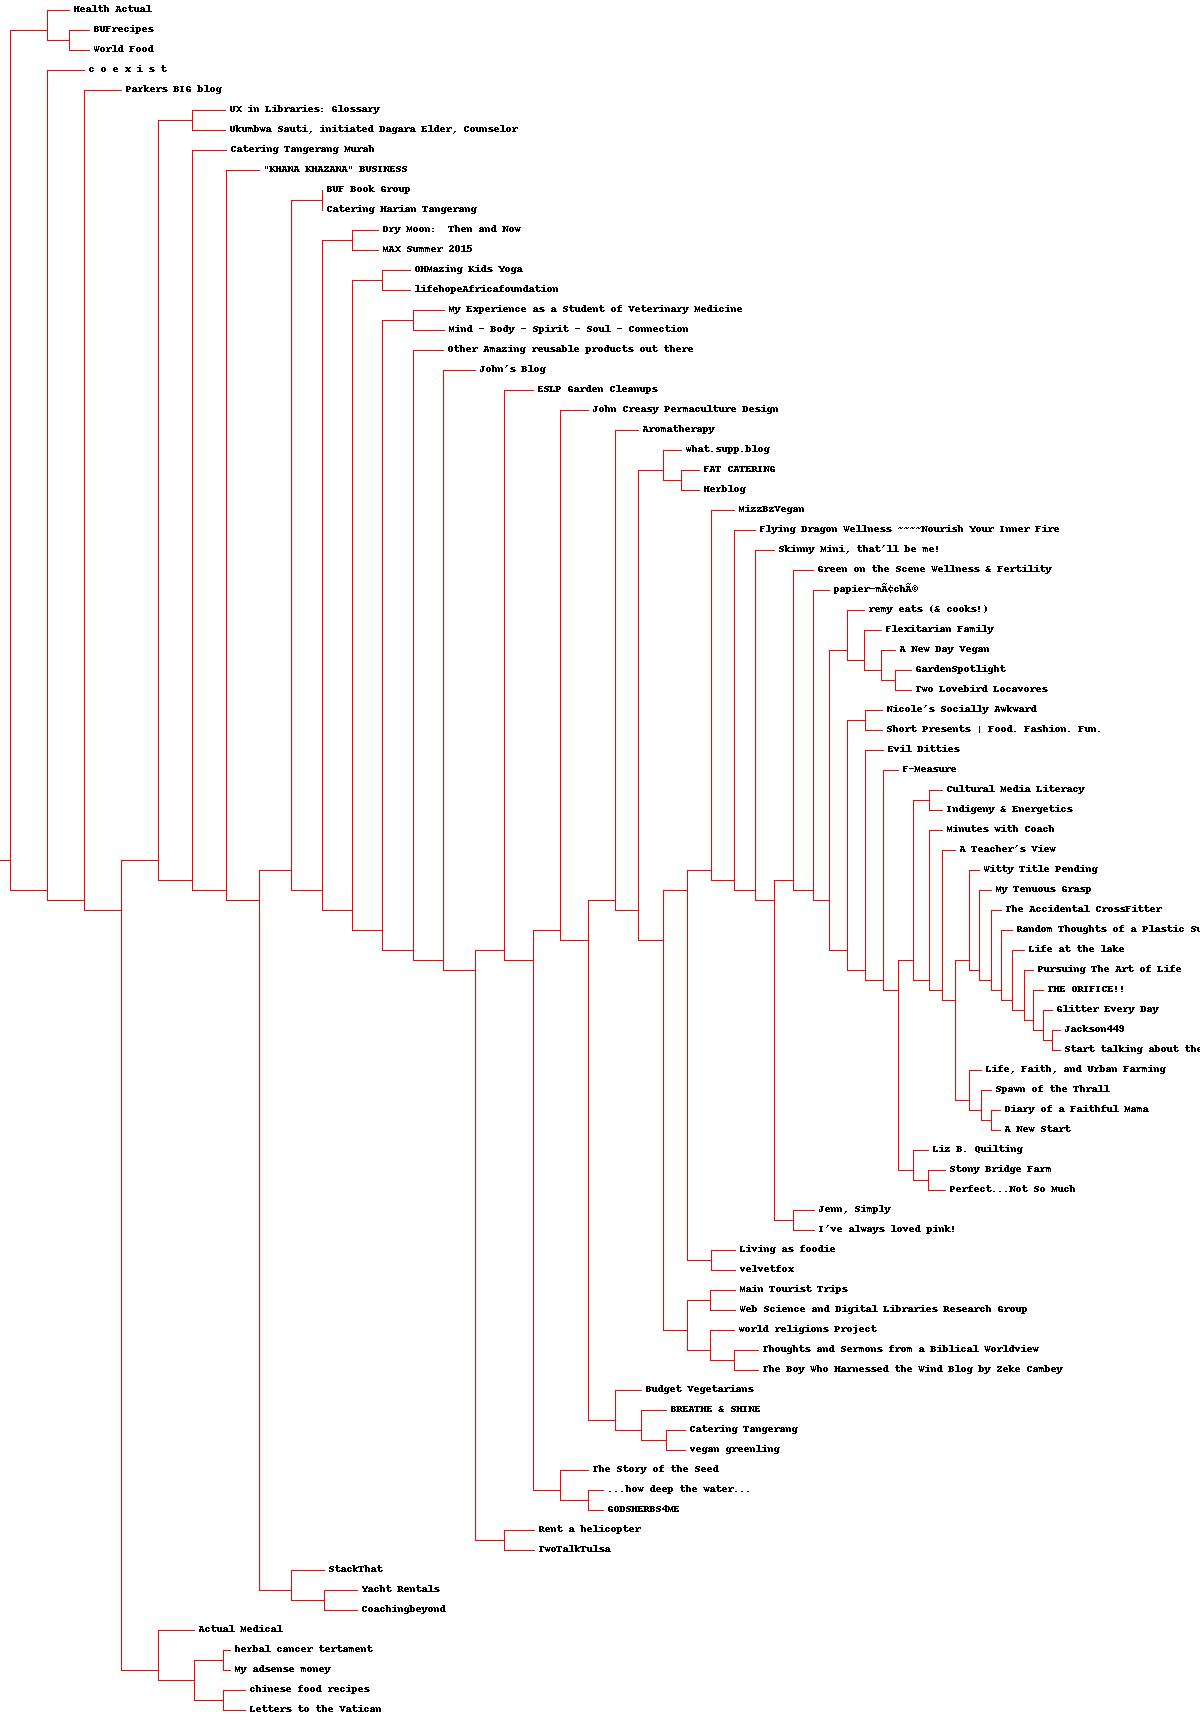
\includegraphics[width=0.8\textwidth]{Dendrogram}
      \caption{Dendogram}
	\end{figure}
	
	
 \end{homeworkProblem}
\clearpage	
\newpage

%----------------------------------------------------------------------------------------
%	PROBLEM 3
%----------------------------------------------------------------------------------------

% To have just one problem per page, simply put a \clearpage after each problem

\begin{homeworkProblem}

Cluster the blogs using K-Means, using k=5,10,20. (see slide 25).  Print the values in each centroid, for each value of k.  
How many iterations were required for each value of k?
 
 
%\problemAnswer{

 \textbf{SOLUTION :}\\

  \begin{enumerate}
 	 \item\textbf{} I coded a  python script \textbf{kmeanclusturing.py} to call the methods from \textbf{clusters.py}
	 \item\textbf{}  I also made use of the tutorial and code available on Github under Programming Collective Intelligence.
   \end{enumerate}	
 
\begin{lstlisting}[language=Python, caption=kmeanclusturing.py]

import clusters
def kMean():
    kMeanValues = [5, 10, 20]
    blogs, colnames, data = clusters.readfile('blogdata.txt')
    for i in kMeanValues:

        kclust, itercount = clusters.kcluster(data, k=i)
        print(kclust)
        f = open("kclust_%d.txt" % i, 'w')
        f.write("Total Number Of Iterations: %d \n" % itercount)
        print(len(kclust))
        clusterCount = 1
        for cluster in kclust:
            i=1
            f.write("---\n")
            f.write("Cluster %d \n" % clusterCount)
            for blogid in cluster:
                f.write(str(i)+".\t"+blogs[blogid] + "\n")
                i+=1
            f.write("\n")
            clusterCount+=1
if __name__ == "__main__":
    kMean()
		
\end{lstlisting}


Results have been uploaded in to GitHub under foler \textbf{3/kclust_5.txt,3/kclust_10.txt and 3/kclust_20.txt}.
It took 11 iterations to create 5 clusters, 5 iterations for 10 cluster and  4 iterations for 20 clusters.

 \end{homeworkProblem}
\clearpage

\newpage

%----------------------------------------------------------------------------------------
%	PROBLEM 4
%----------------------------------------------------------------------------------------

% To have just one problem per page, simply put a \clearpage after each problem

\begin{homeworkProblem}

Use MDS to create a JPEG of the blogs similar to slide 29 of the week 11 lecture.
 How many iterations were required?
 
 
%\problemAnswer{

 \textbf{SOLUTION :}\\

Created a python script \textbf{4/mdsIteration.py} 
 
 \begin{lstlisting}[language=Python, caption=4/mdsIteration.py]
 
 import clusters    


blognames, words, data = clusters.readfile('blogdata.txt')
coords, itercount = clusters.scaledown(data)
clusters.draw2d(coords, labels=blognames, jpeg='mds.jpg')
print ('Iteration count: %d' % itercount)

		
\end{lstlisting}
 
\begin{figure}[h]
  \centering
    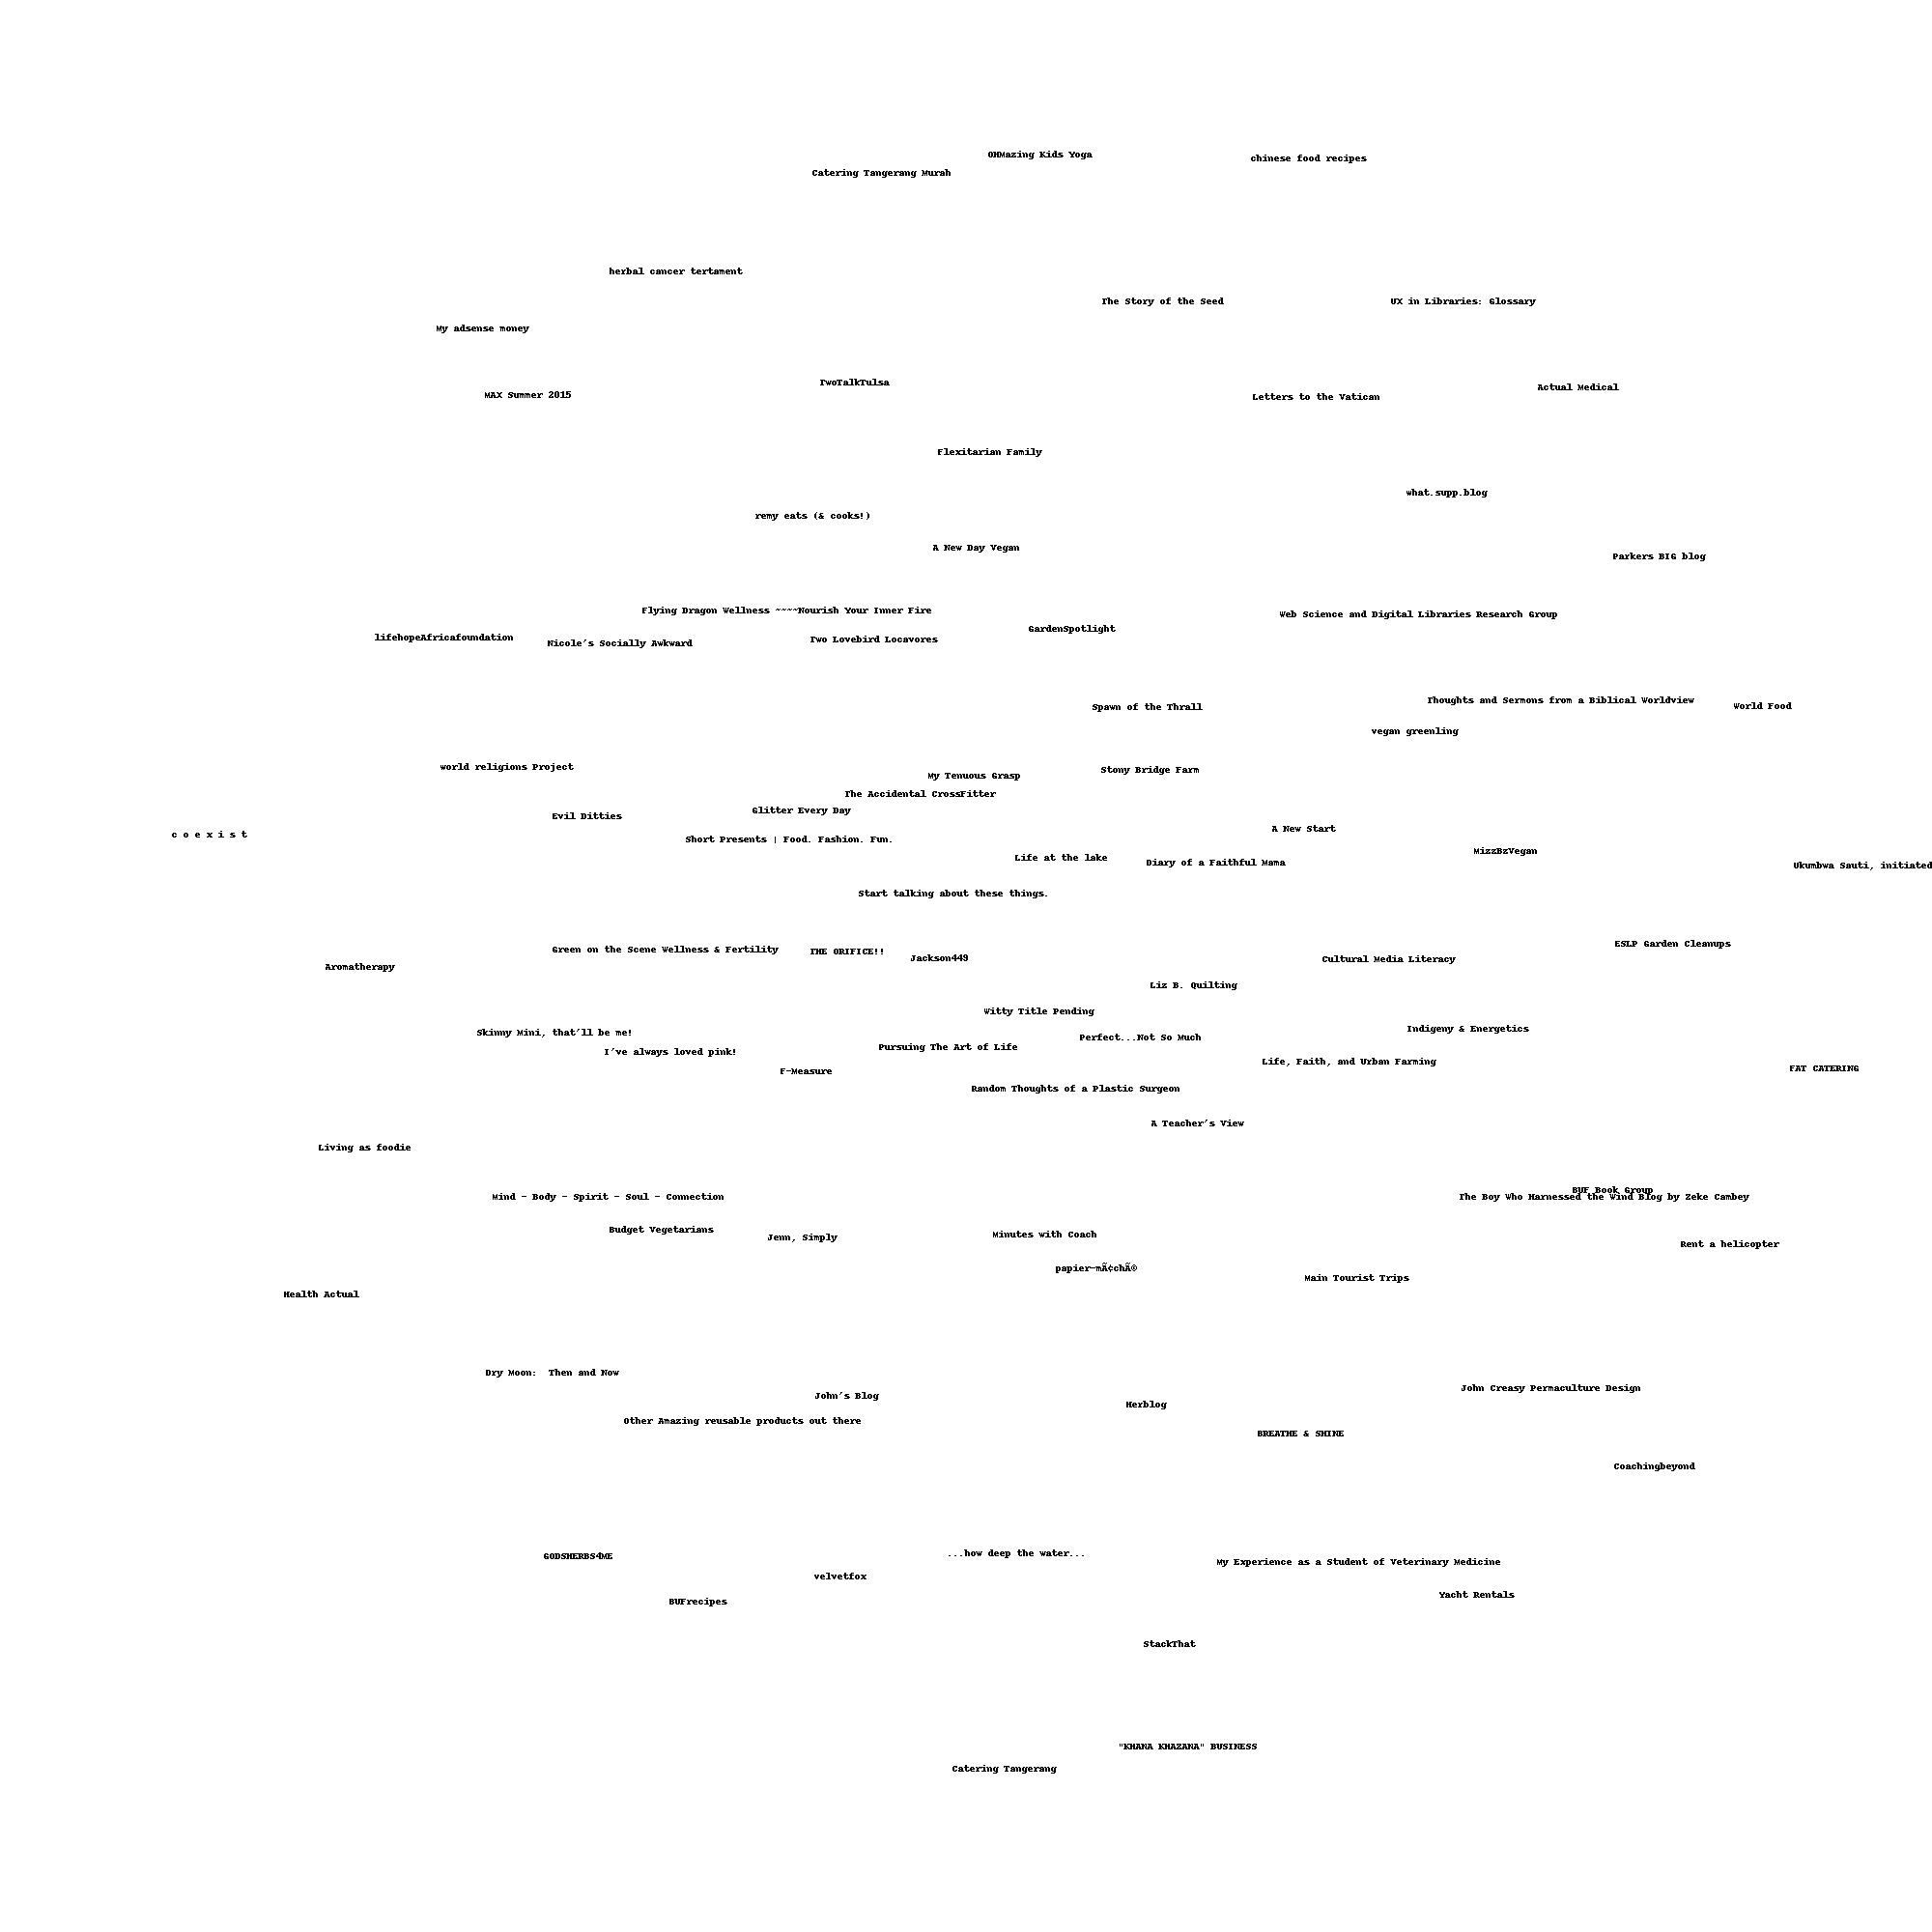
\includegraphics[width=0.7\textwidth]{mds}
      \caption{MDS}
	\end{figure}
	
\begin{figure}[h]
  \centering
    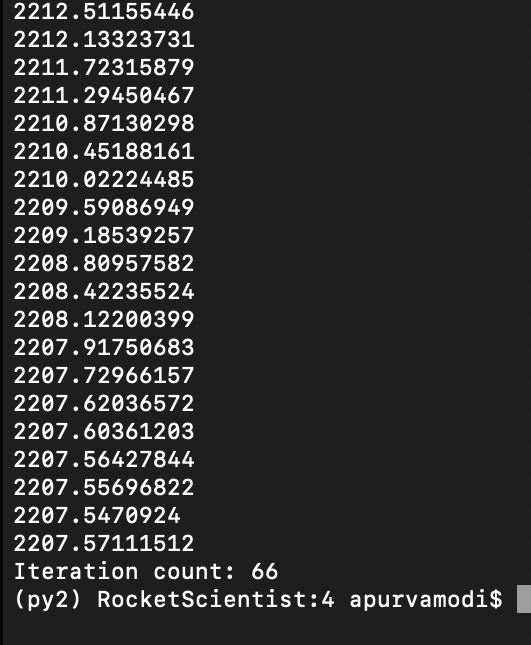
\includegraphics[width=0.7\textwidth]{iterationcount}
      \caption{INumber of iterations}
	\end{figure}
Result was generated with 66 iterations.
	 
 \end{homeworkProblem}
\clearpage
\newpage
 
\textbf{References}
\begin{enumerate}
\item\textbf{} https://github.com/arthur-e/Programming-Collective-Intelligence/tree/master/chapter3
\item\textbf{} https://en.wikipedia.org/wiki/Cluster_analysis
\item\textbf{} https://en.wikipedia.org/wiki/Dendrogram
\item\textbf{} https://en.wikipedia.org/wiki/K-means_clustering
\end{enumerate}
\end{document}
